\PassOptionsToPackage{unicode=true}{hyperref} % options for packages loaded elsewhere
\PassOptionsToPackage{hyphens}{url}
%
\documentclass[]{book}
\usepackage{lmodern}
\usepackage{amssymb,amsmath}
\usepackage{ifxetex,ifluatex}
\usepackage{fixltx2e} % provides \textsubscript
\ifnum 0\ifxetex 1\fi\ifluatex 1\fi=0 % if pdftex
  \usepackage[T1]{fontenc}
  \usepackage[utf8]{inputenc}
  \usepackage{textcomp} % provides euro and other symbols
\else % if luatex or xelatex
  \usepackage{unicode-math}
  \defaultfontfeatures{Ligatures=TeX,Scale=MatchLowercase}
\fi
% use upquote if available, for straight quotes in verbatim environments
\IfFileExists{upquote.sty}{\usepackage{upquote}}{}
% use microtype if available
\IfFileExists{microtype.sty}{%
\usepackage[]{microtype}
\UseMicrotypeSet[protrusion]{basicmath} % disable protrusion for tt fonts
}{}
\IfFileExists{parskip.sty}{%
\usepackage{parskip}
}{% else
\setlength{\parindent}{0pt}
\setlength{\parskip}{6pt plus 2pt minus 1pt}
}
\usepackage{hyperref}
\hypersetup{
            pdftitle={Transfer Mental Health},
            pdfauthor={Alyssa Ortega},
            pdfborder={0 0 0},
            breaklinks=true}
\urlstyle{same}  % don't use monospace font for urls
\usepackage{longtable,booktabs}
% Fix footnotes in tables (requires footnote package)
\IfFileExists{footnote.sty}{\usepackage{footnote}\makesavenoteenv{longtable}}{}
\usepackage{graphicx,grffile}
\makeatletter
\def\maxwidth{\ifdim\Gin@nat@width>\linewidth\linewidth\else\Gin@nat@width\fi}
\def\maxheight{\ifdim\Gin@nat@height>\textheight\textheight\else\Gin@nat@height\fi}
\makeatother
% Scale images if necessary, so that they will not overflow the page
% margins by default, and it is still possible to overwrite the defaults
% using explicit options in \includegraphics[width, height, ...]{}
\setkeys{Gin}{width=\maxwidth,height=\maxheight,keepaspectratio}
\setlength{\emergencystretch}{3em}  % prevent overfull lines
\providecommand{\tightlist}{%
  \setlength{\itemsep}{0pt}\setlength{\parskip}{0pt}}
\setcounter{secnumdepth}{5}
% Redefines (sub)paragraphs to behave more like sections
\ifx\paragraph\undefined\else
\let\oldparagraph\paragraph
\renewcommand{\paragraph}[1]{\oldparagraph{#1}\mbox{}}
\fi
\ifx\subparagraph\undefined\else
\let\oldsubparagraph\subparagraph
\renewcommand{\subparagraph}[1]{\oldsubparagraph{#1}\mbox{}}
\fi

% set default figure placement to htbp
\makeatletter
\def\fps@figure{htbp}
\makeatother

\usepackage{booktabs}
\usepackage{amsthm}
\makeatletter
\def\thm@space@setup{%
  \thm@preskip=8pt plus 2pt minus 4pt
  \thm@postskip=\thm@preskip
}
\makeatother
\usepackage[]{natbib}
\bibliographystyle{apalike}

\title{Transfer Mental Health}
\author{Alyssa Ortega}
\date{2020-05-19}

\begin{document}
\maketitle

{
\setcounter{tocdepth}{1}
\tableofcontents
}
\hypertarget{introduction}{%
\chapter{Introduction}\label{introduction}}

Mental health issues are a prominent and growing concern on college campuses. Although there are many resources on UCLA campus that contribute to student well-being, there are certain populations who may be in need of specialized support. Transfer students in particular encounter several risk factors that may make their transition to a four-year university all the more difficult. However, much of the literature surrounding the transfer experience focuses on academic achievement and pays scant attention to mental health outcomes. This study explores the relationship between being a transfer student and subsequent mental health outcomes. In addition, we explored the effectiveness of campus mental health resources in the student population.

\hypertarget{summary}{%
\section{Summary}\label{summary}}

The UCLA Student Mental Health Study examines how different entry pathways to college education (e.g., transfer or traditional routes) influence student mental health. The study also examines how institutional resources can improve mental health in the face of the existing challenges students encounter.

This is an anonymous online survey taken in one sitting (approximately one hour). The survey is compiled of twenty short questionnaires that ask about demographic information, mental health symptoms, utilization of UCLA resources/communities, student perceptions of UCLA resources/communities, and other experiences you may encounter as a student.

N = 368

\begin{center}\rule{0.5\linewidth}{0.5pt}\end{center}

\hypertarget{keywords}{%
\section{Keywords}\label{keywords}}

transfer student, mental health, risk, resilience, social

\begin{center}\rule{0.5\linewidth}{0.5pt}\end{center}

\hypertarget{background}{%
\section{Background}\label{background}}

The college climate is one in which stress is becoming increasingly prevalent. In fact, the 2008 national survey of counseling survey directors reported an increase in crisis counseling on college campuses (Gallagher, 2008). Reports of depression and suicide are also of increasing concern on college campuses (Mackenzie et al., 2011). Within the college population, there are a subset of students who have transferred to the university from a community college. This population comprises a large portion of UCLA in particular, as the institution offered admission to nearly 5,600 transfer students in the year 2018 alone (Vazquez, 2018). Historically, transfer students come from working class backgrounds and struggle to balance school with their financial responsibilities (Rhine \& Milligan, 2000). Studies show that the transition process from community college to a four-year institution can be difficult because transfers experience potential risk factors such as: low social connectedness, financial issues, and transfer shock (Townsend \& Wilson,2010; Rhine, Milligan, \& Nelson, 2000; Packard et al., 2011; Mehr \& Daltry, 2016; Rhine et al., 2000).

Although we know that social support is vital to a successful college transition, transfer students often live off campus, focus heavily on attaining their degree and have job responsibilities, which further isolate them from socializing with their peers (Townsend \& Wilson, 2010). Unfortunately the literature shows that academic and social factors such as the ones stated above, often accumulate in high attrition rates and student dropout, a phenomenon so popular it is now referred to as ``transfer shock'' (Rhine et al., 2000).

Other studies show that transfer students also experience mental health issues such as depression and anxiety (Au, 2011; Mackenzie et al., 2011; Gallagher, 2008). Although UCLA offers resources such as Counseling and Psychological Services (CAPS), recreational services and programs to ease the transition process, how such programs relate to the transfer student experience or their mental health outcomes remains unknown. Though transfer students are a particularly vulnerable population who experience an abundance of risk factors, the existing literature heavily focuses on transfers academic outcomes with relatively scant attention paid to their mental health outcomes.

Moreover, there is no one study that investigates mental health in the context of social and institutional risk and resilience factors within the transfer student population, which limits the clinical utility of the existing data. In this study, we examined mental health outcomes within first-year transfer and traditional college students at UCLA, and assess interpersonal (e.g., social), and institutional (e.g., psychological service access) risk and resilience factors that could moderate the mental health outcomes.

\begin{center}\rule{0.5\linewidth}{0.5pt}\end{center}

\hypertarget{specific-aims}{%
\section{Specific Aims}\label{specific-aims}}

\begin{enumerate}
\def\labelenumi{\arabic{enumi}.}
\tightlist
\item
  Determine if there are differential risk and resilience factors experienced by first-year transfer students and first-year traditional students at UCLA.
\item
  Identify whether first-year transfer students experience higher mental distress than traditional first-year students at UCLA.
\item
  Establish whether risk factors (which are hypothesized to be higher in transfer students) are associated with poorer mental health outcomes.
\item
  Determine if resilience factors can moderate the association between risk factors and mental health outcomes in the transfer student population.
\end{enumerate}

\hypertarget{methods}{%
\chapter{Methods}\label{methods}}

\hypertarget{measures}{%
\section{Measures}\label{measures}}

\hypertarget{information}{%
\subsection{Information}\label{information}}

\begin{longtable}[]{@{}llll@{}}
\toprule
\begin{minipage}[b]{0.22\columnwidth}\raggedright
Title\strut
\end{minipage} & \begin{minipage}[b]{0.27\columnwidth}\raggedright
Name\strut
\end{minipage} & \begin{minipage}[b]{0.22\columnwidth}\raggedright
Description\strut
\end{minipage} & \begin{minipage}[b]{0.18\columnwidth}\raggedright
Reference\strut
\end{minipage}\tabularnewline
\midrule
\endhead
\begin{minipage}[t]{0.22\columnwidth}\raggedright
Demographics\strut
\end{minipage} & \begin{minipage}[t]{0.27\columnwidth}\raggedright
Transfer Mental Health Demographics\strut
\end{minipage} & \begin{minipage}[t]{0.22\columnwidth}\raggedright
Assesses demographic information including student status, racial identification, and school information\strut
\end{minipage} & \begin{minipage}[t]{0.18\columnwidth}\raggedright
Made by BABLab\strut
\end{minipage}\tabularnewline
\bottomrule
\end{longtable}

\hypertarget{mental-health}{%
\subsection{Mental Health}\label{mental-health}}

\begin{longtable}[]{@{}llll@{}}
\toprule
\begin{minipage}[b]{0.22\columnwidth}\raggedright
Title\strut
\end{minipage} & \begin{minipage}[b]{0.27\columnwidth}\raggedright
Description\strut
\end{minipage} & \begin{minipage}[b]{0.22\columnwidth}\raggedright
Reference\strut
\end{minipage} & \begin{minipage}[b]{0.18\columnwidth}\raggedright
\strut
\end{minipage}\tabularnewline
\midrule
\endhead
\begin{minipage}[t]{0.22\columnwidth}\raggedright
bai\strut
\end{minipage} & \begin{minipage}[t]{0.27\columnwidth}\raggedright
Beck Anxiety Inventory\strut
\end{minipage} & \begin{minipage}[t]{0.22\columnwidth}\raggedright
Assesses anxiety through student self-report of anxiety symptoms within the last month\strut
\end{minipage} & \begin{minipage}[t]{0.18\columnwidth}\raggedright
(Beck et al., 1988)\strut
\end{minipage}\tabularnewline
\begin{minipage}[t]{0.22\columnwidth}\raggedright
dass\strut
\end{minipage} & \begin{minipage}[t]{0.27\columnwidth}\raggedright
Depression Anxiety Stress Scale\strut
\end{minipage} & \begin{minipage}[t]{0.22\columnwidth}\raggedright
Student self-report designed to measure three related negative emotional states: depression, anxiety, and tension/stress\strut
\end{minipage} & \begin{minipage}[t]{0.18\columnwidth}\raggedright
(Lovibond \& Lovibond, 1995)\strut
\end{minipage}\tabularnewline
\begin{minipage}[t]{0.22\columnwidth}\raggedright
pss\strut
\end{minipage} & \begin{minipage}[t]{0.27\columnwidth}\raggedright
Perceived Stress Scale\strut
\end{minipage} & \begin{minipage}[t]{0.22\columnwidth}\raggedright
Assesses how various situations affect perceived stress through self-report of feelings and thoughts over the last month\strut
\end{minipage} & \begin{minipage}[t]{0.18\columnwidth}\raggedright
(Cohen et al., 1983)\strut
\end{minipage}\tabularnewline
\begin{minipage}[t]{0.22\columnwidth}\raggedright
wemwbs\strut
\end{minipage} & \begin{minipage}[t]{0.27\columnwidth}\raggedright
The Warwick-Edinburgh Mental Wellbeing Scale\strut
\end{minipage} & \begin{minipage}[t]{0.22\columnwidth}\raggedright
Assesses mental well-being through self-report by asking participants to indicate which feelings and thoughts best describe their experiences over the last two weeks\strut
\end{minipage} & \begin{minipage}[t]{0.18\columnwidth}\raggedright
(Tennant et al., 2006)\strut
\end{minipage}\tabularnewline
\bottomrule
\end{longtable}

\hypertarget{proposed-risk-factors}{%
\subsection{Proposed Risk Factors}\label{proposed-risk-factors}}

\begin{longtable}[]{@{}llll@{}}
\toprule
\begin{minipage}[b]{0.22\columnwidth}\raggedright
Title\strut
\end{minipage} & \begin{minipage}[b]{0.27\columnwidth}\raggedright
Description\strut
\end{minipage} & \begin{minipage}[b]{0.22\columnwidth}\raggedright
Reference\strut
\end{minipage} & \begin{minipage}[b]{0.18\columnwidth}\raggedright
\strut
\end{minipage}\tabularnewline
\midrule
\endhead
\begin{minipage}[t]{0.22\columnwidth}\raggedright
commuting\_status\strut
\end{minipage} & \begin{minipage}[t]{0.27\columnwidth}\raggedright
Commuting Status Questionnaire\strut
\end{minipage} & \begin{minipage}[t]{0.22\columnwidth}\raggedright
Assesses school commute distance, school commute time, and if the student lives on campus\strut
\end{minipage} & \begin{minipage}[t]{0.18\columnwidth}\raggedright
Made by BABLab\strut
\end{minipage}\tabularnewline
\begin{minipage}[t]{0.22\columnwidth}\raggedright
imposter\_syndrome\strut
\end{minipage} & \begin{minipage}[t]{0.27\columnwidth}\raggedright
Clance Imposter Syndrome Self-Assessment Tool\strut
\end{minipage} & \begin{minipage}[t]{0.22\columnwidth}\raggedright
Assess if the student carries imposter syndrome characteristics and to what extent\strut
\end{minipage} & \begin{minipage}[t]{0.18\columnwidth}\raggedright
(Clance, 1985)\strut
\end{minipage}\tabularnewline
\begin{minipage}[t]{0.22\columnwidth}\raggedright
dmi\strut
\end{minipage} & \begin{minipage}[t]{0.27\columnwidth}\raggedright
Dweck Mindset Instrument\strut
\end{minipage} & \begin{minipage}[t]{0.22\columnwidth}\raggedright
Assesses if the student has a fixed or growth mindset\strut
\end{minipage} & \begin{minipage}[t]{0.18\columnwidth}\raggedright
(Dweck, 2016)\strut
\end{minipage}\tabularnewline
\begin{minipage}[t]{0.22\columnwidth}\raggedright
financial\_burden\strut
\end{minipage} & \begin{minipage}[t]{0.27\columnwidth}\raggedright
Financial Burden Questionnaire\strut
\end{minipage} & \begin{minipage}[t]{0.22\columnwidth}\raggedright
Assesses to what extent the student feels financially insecure\strut
\end{minipage} & \begin{minipage}[t]{0.18\columnwidth}\raggedright
Made by BABLab\strut
\end{minipage}\tabularnewline
\begin{minipage}[t]{0.22\columnwidth}\raggedright
familial\_obligation\strut
\end{minipage} & \begin{minipage}[t]{0.27\columnwidth}\raggedright
Familial Obligation Questionnaire\strut
\end{minipage} & \begin{minipage}[t]{0.22\columnwidth}\raggedright
Assesses level of familial responsibilities\strut
\end{minipage} & \begin{minipage}[t]{0.18\columnwidth}\raggedright
Made by BABLab\strut
\end{minipage}\tabularnewline
\begin{minipage}[t]{0.22\columnwidth}\raggedright
transfer\_shock\strut
\end{minipage} & \begin{minipage}[t]{0.27\columnwidth}\raggedright
Transfer Shock Questionnaire\strut
\end{minipage} & \begin{minipage}[t]{0.22\columnwidth}\raggedright
Assesses how smooth the student perceives their transition and how prepared they felt for UCLA rigor\strut
\end{minipage} & \begin{minipage}[t]{0.18\columnwidth}\raggedright
Made by BABLab\strut
\end{minipage}\tabularnewline
\bottomrule
\end{longtable}

\hypertarget{proposed-resilience-factors}{%
\subsection{Proposed Resilience Factors}\label{proposed-resilience-factors}}

\begin{longtable}[]{@{}llll@{}}
\toprule
\begin{minipage}[b]{0.22\columnwidth}\raggedright
Title\strut
\end{minipage} & \begin{minipage}[b]{0.27\columnwidth}\raggedright
Description\strut
\end{minipage} & \begin{minipage}[b]{0.22\columnwidth}\raggedright
Reference\strut
\end{minipage} & \begin{minipage}[b]{0.18\columnwidth}\raggedright
\strut
\end{minipage}\tabularnewline
\midrule
\endhead
\begin{minipage}[t]{0.22\columnwidth}\raggedright
grittiness\strut
\end{minipage} & \begin{minipage}[t]{0.27\columnwidth}\raggedright
Angela Duckworth Grit Scale\strut
\end{minipage} & \begin{minipage}[t]{0.22\columnwidth}\raggedright
Assesses passion and perseverance\strut
\end{minipage} & \begin{minipage}[t]{0.18\columnwidth}\raggedright
(Duckworth et al., 2007)\strut
\end{minipage}\tabularnewline
\begin{minipage}[t]{0.22\columnwidth}\raggedright
mpss\strut
\end{minipage} & \begin{minipage}[t]{0.27\columnwidth}\raggedright
Multidimensional Scale of Perceived Social Support\strut
\end{minipage} & \begin{minipage}[t]{0.22\columnwidth}\raggedright
Assesses feeling of support from family, friends, and significant others\strut
\end{minipage} & \begin{minipage}[t]{0.18\columnwidth}\raggedright
(Zimet et al., 1988)\strut
\end{minipage}\tabularnewline
\begin{minipage}[t]{0.22\columnwidth}\raggedright
psqi\strut
\end{minipage} & \begin{minipage}[t]{0.27\columnwidth}\raggedright
The Pittsburgh Sleep Quality Index\strut
\end{minipage} & \begin{minipage}[t]{0.22\columnwidth}\raggedright
Assesses quality and patterns of sleep\strut
\end{minipage} & \begin{minipage}[t]{0.18\columnwidth}\raggedright
(Buysse et al., 1989)\strut
\end{minipage}\tabularnewline
\begin{minipage}[t]{0.22\columnwidth}\raggedright
financial\_wellbeing\strut
\end{minipage} & \begin{minipage}[t]{0.27\columnwidth}\raggedright
CFPB Financial Well-Being Scale Questionnaire\strut
\end{minipage} & \begin{minipage}[t]{0.22\columnwidth}\raggedright
Assesses feelings of financial security and concern\strut
\end{minipage} & \begin{minipage}[t]{0.18\columnwidth}\raggedright
(Consumer Financial Protection Bureau)\strut
\end{minipage}\tabularnewline
\begin{minipage}[t]{0.22\columnwidth}\raggedright
free-time\strut
\end{minipage} & \begin{minipage}[t]{0.27\columnwidth}\raggedright
Free-time Questionnaire\strut
\end{minipage} & \begin{minipage}[t]{0.22\columnwidth}\raggedright
Assesses amount of time student engages in time for themselves and things they enjoy\strut
\end{minipage} & \begin{minipage}[t]{0.18\columnwidth}\raggedright
Made by BABLab\strut
\end{minipage}\tabularnewline
\begin{minipage}[t]{0.22\columnwidth}\raggedright
dedication\strut
\end{minipage} & \begin{minipage}[t]{0.27\columnwidth}\raggedright
Dedication Questionnaire\strut
\end{minipage} & \begin{minipage}[t]{0.22\columnwidth}\raggedright
Assesses how devoted the student is to their studies and school goals\strut
\end{minipage} & \begin{minipage}[t]{0.18\columnwidth}\raggedright
Made by BABLab\strut
\end{minipage}\tabularnewline
\begin{minipage}[t]{0.22\columnwidth}\raggedright
caps\strut
\end{minipage} & \begin{minipage}[t]{0.27\columnwidth}\raggedright
Satisfaction with UCLA Counseling and Psychological Services (CAPS) Questionnaire\strut
\end{minipage} & \begin{minipage}[t]{0.22\columnwidth}\raggedright
Assesses use of CAPS, how satisfied they were with the services, and how accessible they feel the services are to the community\strut
\end{minipage} & \begin{minipage}[t]{0.18\columnwidth}\raggedright
Made by BABLab\strut
\end{minipage}\tabularnewline
\begin{minipage}[t]{0.22\columnwidth}\raggedright
tsp\strut
\end{minipage} & \begin{minipage}[t]{0.27\columnwidth}\raggedright
Satisfaction of UCLA Transfer Student Program (TSP) Questionnaire\strut
\end{minipage} & \begin{minipage}[t]{0.22\columnwidth}\raggedright
Assesses use of TSP, how satisfied they were with the program, possible barriers to attendance and if the program facilitated their transition\strut
\end{minipage} & \begin{minipage}[t]{0.18\columnwidth}\raggedright
Made by BABLab\strut
\end{minipage}\tabularnewline
\begin{minipage}[t]{0.22\columnwidth}\raggedright
club\_involvement\strut
\end{minipage} & \begin{minipage}[t]{0.27\columnwidth}\raggedright
Campus Club Involvement Questionnaire\strut
\end{minipage} & \begin{minipage}[t]{0.22\columnwidth}\raggedright
Assesses feelings of campus connectedness through club involvement and possible barriers to access\strut
\end{minipage} & \begin{minipage}[t]{0.18\columnwidth}\raggedright
Made by BABLab\strut
\end{minipage}\tabularnewline
\begin{minipage}[t]{0.22\columnwidth}\raggedright
recreational\_activities\strut
\end{minipage} & \begin{minipage}[t]{0.27\columnwidth}\raggedright
Use of UCLA Recreational Activities Questionnaire\strut
\end{minipage} & \begin{minipage}[t]{0.22\columnwidth}\raggedright
Assesses utilization of campus recreational facilities and its relationship to feelings of stress\strut
\end{minipage} & \begin{minipage}[t]{0.18\columnwidth}\raggedright
Made by BABLab\strut
\end{minipage}\tabularnewline
\bottomrule
\end{longtable}

\begin{center}\rule{0.5\linewidth}{0.5pt}\end{center}

\hypertarget{procedure}{%
\section{Procedure}\label{procedure}}

Students answered surveys anonymously online through RedCap. These surveys assess domains of student experience, as well as potential outside barriers that may inhibit successful transition to UCLA. In addition, the questions ask the participant to document their experiences or use of certain campus resources that may buffer against the relationship between being a transfer student and poor mental health outcomes. The questions also assess the participants' mental health through a variety of questionnaires which ask about the participants' thoughts, feelings, and experiences.

\hypertarget{questionnaire-order}{%
\subsection{Questionnaire Order}\label{questionnaire-order}}

\begin{enumerate}
\def\labelenumi{\arabic{enumi}.}
\tightlist
\item
  Demographics
\item
  Pss
\item
  Bai
\item
  Club\_involvement 
\item
  Psqi
\item
  Dass
\item
  Wemwbs
\item
  Commuting\_status
\item
  Caps
\item
  Dedication
\item
  Dmi
\item
  Familial\_obligation
\item
  Financial\_burden
\item
  Financial\_well\_being
\item
  Free\_time
\item
  Fsp
\item
  Tsp
\item
  Grittiness
\item
  Imposter\_syndrome
\item
  Perceived\_social\_support
\item
  Recreational\_activities
\item
  Transfer\_shock
\end{enumerate}

\hypertarget{attention-checks}{%
\subsection{Attention Checks}\label{attention-checks}}

\begin{enumerate}
\def\labelenumi{\arabic{enumi}.}
\tightlist
\item
  Financial\_well\_being:
  \emph{It is crucial that you are paying full attention to the study. Please tick ``Very well''}
\item
  Perceived\_social\_support:
  \emph{To ensure that you are giving this study your complete attentiveness, please select ``Strongly Agree''}
\item
  Caps:
  \emph{For this question, please click number 3}
\end{enumerate}

\hypertarget{recruitment}{%
\subsection{Recruitment}\label{recruitment}}

Participants were recruited through one of two methods: For Psychology affiliated students, recruitment occurred through SONA systems, which is an online system used to schedule and manage the UCLA Psychology Department human subject pool. In addition, to obtain data from the wider (non-Psychology) community at UCLA, we also had a non-SONA based version of the questionnaire (using RedCap). The survey was open for the Spring 2020 term, and all survey respondents during those quarters were included in the final analyses.

The following materials were used:

\textbf{Flyer:}

\begin{figure}
\centering
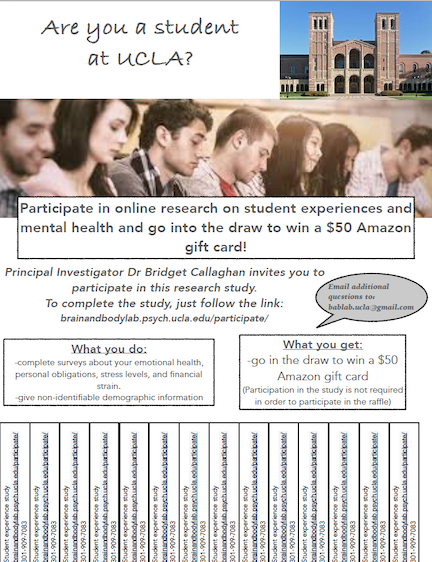
\includegraphics{images/tmh_flyer.png}
\caption{}
\end{figure}

\textbf{Video Advertisement:}

\begin{center}\rule{0.5\linewidth}{0.5pt}\end{center}

\hypertarget{references}{%
\chapter{References}\label{references}}

Au, J. (2011). A Longitudinal Study Examining the Role of Social Connectedness in the Course
of Depressive Symptoms: An Evaluation of Transfer and Freshman
Students(Unpublished doctoral dissertation ). University of Michigan.

Beck, A. T., \& Steer, R. A. (1993). Beck Anxiety Inventory Manual . San Antonio, TX: The
Psychological Corporation Harcourt Brace \& Company.

Buysse, D. J., Reynolds, C. F., Monk, T. H., Berman, S. R., \& Kupfer, D. J. (1989). The
Pittsburgh Sleep Quality Index: A new instrument for psychiatric practice and research.
Psychiatry Research, 28 (2), 193--213. \url{https://doi.org/10.1016/0165-1781(89)90047-4}

Clance, P. R. (1986). The impostor phenomenon: when success makes you feel like a fake . New
York: Bantam Books.

Cohen, S., Kamarck, T., and Mermelstein, R. (1983). A global measure of perceived stress.
Journal of Health and Social Behavior , 24, 386-396.
College Transfer Pathway. Journal of Women and Minorities in Science and Engineering, 17 (2),129-147. \url{doi:10.1615/jwomenminorscieneng.2011002470}

Duckworth, A. L., Peterson, C., Matthews, M. D., \& Kelly, D. R. (2007). Grit: Perseverance and passion for long-term goals. Journal of Personality and Social Psychology , 92 (6),
1087--1101. \url{doi:10.1037/0022-3514.92.6.1087}

Dweck, C. S. (2006). Mindset: The new psychology of success. New York: Random House.
Find out your financial well-being. (n.d.). Retrieved December 10, 2019, from
\url{https://www.consumerfinance.gov/consumer-tools/financial-well-being/}.

Gallagher, R. P. (2008). National Survey of Counseling Directors. The American College
Counseling Association.

Lovibond, S. H., \& Lovibond, P. F. (1995). Manual for the Depression Anxiety Stress Scales
(2nd ed.). Sydney: Psychology Foundation of Australia.

Mackenzie, S., Wiegel, J. R., Mundt, M., Brown, D., Saewyc, E., Heiligenstein, E., \ldots{} Fleming,M. (2011). Depression and suicide ideation among students accessing campus health
care. American Journal of Orthopsychiatry , 81 (1), 101--107. \url{doi:10.1111/j.1939-0025.2010.01077}.

Mehr, K. E., \& Daltry, R. (2016). Examining Mental Health Differences between Transfer and
Nontransfer University Students Seeking Counseling Services. Journal of College
Student Psychotherapy, 30 (2), 146-155. \url{doi:10.1080/87568225.2016.1140996}

Packard, B. W., Gagnon, J. L., Labelle, O., Jeffers, K., \& Lynn, E. (2011). Womens Experiences In The Stem Community Rhine, T. J., Milligan, D. M., Nelson, L. R. (2000). Alleviating Transfer Shock: Creating An Environment For More Successful Transfer Students. Community College Journal of Research and Practice, 24 (6), 443-453. \url{doi:10.1080/10668920050137228}

Tennant, R., Hiller, L., Fishwick, R., Platt, S., Joseph, S., Weich, S., Parkinson, J., Secker, J., \& Stewart-Brown, S. (2007). The Warwick-Edinburgh Mental Well-being Scale
(WEMWBS): Development and UK validation. Health and Quality of Life Outcomes, 5,
Article 63. \url{https://doi.org/10.1186/1477-7525-5-63}

Townsend, B. K., \& Wilson, K. B. (2009). The Academic and Social Integration of Persisting
Community College Transfer Students. \url{doi:10.2190/CS.10.4.a}

Vazquez , R. (2018, July 11). UCLA offers freshman admission to 16,000, increases offers to
transfer students. Retrieved from
\url{http://newsroom.ucla.edu/releases/ucla-offers-freshman-admission-to-16-000-increases-offers-to-transfer-students}

Zimet, G.D., Dahlem, N.W., Zimet, S.G. \& Farley, G.K. (1988). The Multidimensional Scale of
Perceived Social Support. Journal of Personality Assessment , 52, 30-41.

\bibliography{book.bib,packages.bib,ref.bib}

\end{document}
